\documentclass[a4paper,11pt]{article}
\usepackage[a4paper]{geometry}
\usepackage{polski}
\usepackage[polish]{babel}
\usepackage[utf8]{inputenc}

\usepackage{indentfirst} %taby na początku
\usepackage{graphicx} %dodawanie obrazków
\usepackage{subcaption}

\usepackage{lastpage} %znacznik ostatniej strony
\usepackage{fancyhdr} %odblokowanie wyglądu fancy
\usepackage{hyperref} %hiperłącza
\usepackage{float} %latające napisy
\usepackage{chngcntr} %zmiana countera

\usepackage{amsmath} %konieczne do matmy
\usepackage{amsfonts} %konieczne do czcionek mathbb
\usepackage{mathrsfs} %konieczne do czcionek mathscr
\usepackage{relsize}

\usepackage{tikz} %rysowanie obrazów
\usepackage{pgfplots}
\usepackage{siunitx}
\usepackage{rotating}
\usepackage{xcolor}

\usepackage{adjustbox}
\usepackage{multirow}
\usepackage{tabularx}
\usepackage{chngpage}

\usepackage{listings}
\usepackage[paper=portrait,pagesize]{typearea}

\usetikzlibrary{arrows.meta,arrows}
\lstset{basicstyle=\small\ttfamily,breaklines=true,tabsize=2,numbers=left,showstringspaces=false,commentstyle=\color{red},keywordstyle=\color{blue}}
%head & foot
\counterwithin*{section}{part}
\pagestyle{fancy}
\title{Notatki}
\author{Mateusz Łuczak}
\date{}
\setlength\parindent{24pt}
\setlength{\headheight}{16pt}
\lhead{}
\rhead{}
\rfoot{str. \thepage/\pageref{LastPage}}
\cfoot{}
%do linii na górze
\renewcommand{\headrulewidth}{0pt}

\pgfplotsset{compat=newest}
\usepgfplotslibrary{units}

%\KOMAoptions{paper=landscape,pagesize}
%\recalctypearea
%end of preamble
\begin{document}
%\maketitle
%\thispagestyle{empty}
%\newpage

%\tableofcontents
%\pagenumbering{arabic}
%\newpage

\thispagestyle{empty}
\begin{center}
	\textsc{\LARGE Politechnika Warszawska}\\[1.5cm]

	\textsc{\Large Wydział Elektryczny}\\[0.5cm]

	\textsc{\large Informatyka Stosowana}\\[2cm]

	\rule{\linewidth}{0.5mm}

	\textsc{\Large Sprawozdanie z projektu 1}\\[0.5cm]

	\textit{Testowanie oprogramowania} (1DI1542)

	\rule{\linewidth}{0.5mm}\\[3cm]

	\normalsize
	Michał Bogusz
	
	Krzysztof Dąbrowski

	Adrian Krzeszewski

	Mateusz Łuczak

	Paweł Osiński
\end{center}

\newpage
\pagenumbering{arabic}
\tableofcontents
\newpage

\section{Opis projektu}
Podczas wykonywania projektu stworzono prostą aplikację służącą do zarządzania budżetem domowym. Wszyscy użytkownicy systemu -- domownicy -- mają możliwość edytowania listy zakupów oraz raportowania dokonanych zakupów.

\section{Baza danych}
Zaprojektowana do tego projektu baza danych pozwala wypełnić wszystkie opisane założenia. Składa się z 4 tabel zawierających rekordy reprezentujące:
\begin{itemize}
	\item członków rodziny;
	\item produkty;
	\item wykonane zakupy;
	\item listę zakupów.
\end{itemize}

\begin{figure}[h!]
	\centering
	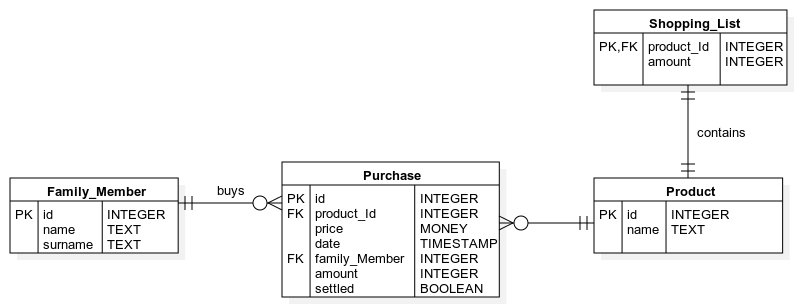
\includegraphics[scale=0.5]{P1.png}
	\caption{Model bazy danych}
	\label{fig:p1}
\end{figure}

\section{Funkcjonalność programu}
W programie, użytkownik ma dostęp do następujących funkcji:
\begin{itemize}
	\item dodawanie członków rodziny
	\item dodawanie produktów
	\item rejestrowanie zakupów
	\item wyświetlanie listy członków rodziny
	\item wyświetlanie listy produktów
	\item wyświetlanie listy zakupów
	\item wyświetlanie raportu zakupów
	\item usuwanie członków rodziny
	\item usuwanie produktów
\end{itemize}

\section{Architektura systemu}
Projekt został wykonany z użyciem silnika Docker. Baza danych implementujących standard SQL jest zarządzana za pomocą systemu PostgreSQL. Baza jest uruchamiana jako kontener silnika Docker. Warstwa aplikacyjna projektu została wykonana w języku Java. W celu zapewnienia sprawnego współdziałania napisanych skryptów z systemem PostgreSQL użyty został framework Hibernate, do którego dostęp został zapewniony poprzez metody Javy, napisane ściśle według paradygmatu CRUD. Do testów użyto biblioteki JUnit, a do zapewnienia konsolidacji wszystkich elementów -- narzędzia Maven.

\section{Testy}
Część aplikacyjna została przetestowana ze szczególnym naciskiem na sprawdzenie poprawności zaimplementowania metod opartych na paradygmacie CRUD. Wszystkie metody implementujące jego założenia zostały opatrzone testami jednostkowymi, które uwzględniają scenariusze mające na celu sprawdzenie kluczowych funkcjonalności aplikacji.

Ponieważ CRUD jest paradygmatem, który z swojej definicji zapewnia odpowiednie reguły współpracy różnych warstw programu, jego testowanie -- mimo, że może być przeprowadzane ściśle pod kątem czterech składowych paradygmatu -- \textbf{nie może się odbyć w oderwaniu od całości systemu}. Warto jednak zauważyć, że z powodu mnogości rozwiązań, za pomocą których możliwe jest powiązanie aplikacji z bazą danych, możliwe jest takie stworzenie testów, aby sprawdzać poprawność CRUD niezależnie od standardu i sposobu komunikacji z bazą danych. Takie rozwiązanie wydaje się atrakcyjnym sposobem testowania poprawności komunikacji, gdyż aplikacja może korzystać z różnych typów baz danych lub sposobów łączenia się z bazami, jak również w sytuacjach, gdy brana jest pod uwagę możliwość zmiany obszaru bazodanowego projektu w przyszłości.

\section{Podsumowanie}
Użycie silnika Docker pozwala na szybkie i wygodne zbudowanie systemu, który charakteryzuje się wysoką przenaszalnością. Kontenery Docker zapewniają modularną budowę systemu, co przekłada się na większą elastyczność, oraz pozwala zmniejszyć liczbę potrzebnych do zainstalowania oraz skonfigurowania narzędzi, przed przystąpieniem do pracy nad projektem. Paradygmat CRUD okazuje się przydatny podczas tworzenia połączenia między warstwą aplikacyjną projektu a bazą danych, gdyż ułatwia wyznaczenie zakresu zadań jakie muszą być wykonane aby zbudować kompletny system. Framework Hibernate pozwala na wygodne mapowanie obiektów w języku Java na wiersze bazodanowe. Takie rozwiązanie zapewnia wygodniejszy sposób zarządzania danymi, oraz nie nakłada na użytkownika obowiązku znajomości struktury języka SQL.
\end{document}